Since the work of pioneers of neuropsychology, it has been observed that many neurological and psychiatric disorders can be described as dysconnectivity syndromes~\cite{catani2005}.
The emergence of symptoms or functional impairment in these disorders can be related to the damage or abnormal integration of spatially distributed brain regions that would normally constitute a large-scale network subserving function.
Abnormal patterns of brain functional connectivity have been consistently observed in patients affected by Schizophrenia (SZ) using functional MRI and other neuroimaging methods.
Graph theoretical approaches have been applied to study defective interactions and modular organization in networks of distributed brain areas, perhaps a result of dysfunctional conscious integration in SZ.

As shown in the previous chapters, current graph analysis methods suffer from a fundamental resolution limit, as they fail to detect modules that are smaller than a scale determined by the entire connectivity network.

In this chapter, a first application of Asymptotical Surprise optimization is demonstrated for the study of the modular organization of resting state functional connectivity networks in a large cohort of SZ patients, and in matched healthy controls.
These preliminary results have been obtained with the collaboratiom of my colleague Cécile Bordier at the Center for Neuroscience and Cognitive Systems of ``Istituto Italiano di Tecnologia'' in Rovereto (Italy).

Application of the methodological advances introduced in this work showed a substantial fragmentation and reorganization involving primary sensory, auditory and visual areas in SZ patients. Conversely, frontal and prefrontal areas related with higher cognitive functions appeared to be less affected, with changes involving mostly language-processing regions.
These findings, not yet published, support the hypothesis that cognitive deficits in SZ may be driven by impairments in basic perceptual processes that localize to primary sensory brain regions.


%%%%%%%%%%%%%%%%%%%%%%%%%%%%%%%%%%%%%%%%%%%%%%%%%%%%%%%%%%%%%%%%%%%%%%%%%%%%%%
%%%%%%%%%%%%%% FUNCTIONAL CONNECTIVITY IN SCHIZOPHRENIA %%%%%%%%%%%%%%%%%%%%%%
%%%%%%%%%%%%%%%%%%%%%%%%%%%%%%%%%%%%%%%%%%%%%%%%%%%%%%%%%%%%%%%%%%%%%%%%%%%%%%
\section{Functional connectivity in schizophrenia}
Schizophrenia has been associated with aberrant functional connectivity as measured by neuroimaging methods in a number of studies~\cite{friston1995,bullmore1998,liang2006,liu2008,calhoun2009,alexander-bloch2010,alexander-bloch2012,alexander-bloch2013}.
This growing evidence is in keeping with the disconnectivity hypothesis of Schizophrenia that posits that the core dysfunction of this disease may correspond to weakening of the functional interactions between specialized brain areas~\cite{ellison-wright2009,fornito2009,kubicki2005}, resulting in defective integration of activity in distributed networks and in cognitive disintegration~\cite{tononi2000}.
Indeed, psychotic symptoms akin to those of schizophrenia, including hallucinations and delusions, are also observed in certain neurological disorders that involve disruption of corticocortical and corticosubcortical connections~\cite{hyde1992}.
Understanding the nature of connectivity alterations in SZ patients and their effects on brain functional integration may provide important insights into the etiology of this devastating disease, as well as potential diagnostic or prognostic markers.

To this end, graph theoretical approaches have been proposed as a powerful framework to assess topological features of functional connectivity networks~\cite{bassett2006,bullmore2009,kaiser2011,stam2007}.
Several alterations in graph-related metrics of resting state connectivity have been identified in schizophrenia patients, including reduction in global network efficiency~\cite{liu2008,bullmore2009,bassett2008}, small worldness~\cite{liu2008,anderson2013,yu2011} and rich-club organization of high-connectivity nodes~\cite{vandenheuvel2013}.

Several studies have assessed the modular structure of resting state functional connectivity networks derived from functional MRI in Schizophrenia patients compared to healthy controls~\cite{liu2008,alexander-bloch2010,lerman-sinkoff2016}.
Disrupted modular organization and reduction in Modularity, a measure of segregation of functional modules within the network, was found in Childhood Onset Schizophrenia~\cite{alexander-bloch2010}.
Reduced Modularity was associated with a proportional increase in inter-cluster edges and decrease in intra-cluster edges~\cite{alexander-bloch2012}.
Lerman-Sinkoff et al.~\cite{lerman-sinkoff2016} reported similar community structures in adult schizophrenia patients and healthy subjects under stringent control of potential sources of imaging artifacts, with small but significant alterations of node community membership in specific networks.
Yu et al.~\cite{yu2012} found reduced overall connectivity strength and a larger number of communities in the patients' group (6 in SZ subjects vs 5 in healthy controls).

These pioneering investigations provide important indications that the modular organization of functional connectivity networks may be altered in patients affected by schizophrenia.
However, graph theory as applied to the study of brain networks is still in its infancy, and several methodological and conceptual issues that are still open may have affected early studies.

In the previous chapters I have shown that the resolution limit severely hampered the ability to resolve the modular organization of human brain connectivity networks, and to capture their complex community structure.
This pervasive limit is likely to have biased previous studies in clinical populations, and may have prevented detection of differences in the organization of functional connectivity in patients and controls at a finer scale.
Indeed, even though previous studies in SZ populations systematically report substantial reduction in functional connectivity strength and modularity compared to healthy controls, differences in the number, size and boundaries of functional modules appear to be inconsistent across studies and dependent on the specific clustering approach that was adopted.

The deleterious effects of the resolution limit propagate to the evaluation of important topological parameters that depend on the network's community structure.
These include within-module-degree and participation coefficient, parameters that enable the identification of highly-connected nodes, or hubs, responsible for the integration and efficient exchange of information between modules~\cite{bullmore2009}.

\section{Asymptotical Surprise optimization on schizophrenic patients}
Here, capitalizing on these important methodological advances discussed in the previous chapters, we applied Asymptotical Surprise to resolve and compared the modular structures of resting state functional connectivity networks in two cohorts of 78 schizophrenia subjects and 91 controls.

In contrast with previous studies, we have found profound changes in the resting state brain connectivity structure of schizophrenia patients, with a substantial functional reorganization reflecting both fragmentation and merging of functional modules.
Additionally, we investigated alterations in node-wise participation coefficients and the resulting rearrangement of brain integrative regions in patients.

\subsection{Material and methods}
MRI data were downloaded for 78 people with schizophrenia strict (SCZ) (64 males, 14 females) and 91 healthy controls (CON) (65 males, 26 females) from the open COBRE database \url{http://fcon_1000.projects.nitrc.org/indi/retro/cobre.html}.
Ranging ages going from 18 to 65 years in both groups.
All the subjects in the COBRE were screened and excluded if they had history of neurological disorder, history of mental retardation, history of severe head trauma with more than 5 minute loss of consciousness, history of substance abuse or dependence within the last 12 months.
Ethical statements are contained in the original publication of this dataset.
Images were acquired with a Siemens MIND TRIO 3T scanner equipped for echo-planar imaging (EPI).
Echo-planar imaging was used for resting state fMRI data collection with (Repetition Time) TR=2s, (Echo Time) TE=29ms, matrix size: 64x64, slices=33, voxel size=$3 \times 3 \times 4$ mm$^3$ (for more details see~\cite{cetin2014}).
A total of 150 volumes of functional images were obtained for all the subjects except one (this subject was excluded from the present study).
The data were pre-processed using SPM8 (Wellcome Trust Centre for Neuroimaging, London, UK).
After discarding the four initial volumes, the remaining volumes were slice-timed, head-motion realigned and normalized to the standard MNI EPI template space (voxel-size re-sampled to $3 \times 3 \times 3$ mm$^3$).
Then, for each participant, 638 regional mean time series were computed by averaging the voxel time series within each of the parcellized areas of~\cite{crossley2013a} template. 
Finally, after regressing the movement parameters from each areas signal, we estimated the connectivity matrix by computing pairwise inter-regional correlation for each participation.
In order to have a connectivity matrix by population, we Fisher-transformed individual correlation matrix and average them by group in order to get an adjacency matrix.
In order to determine the optimal modular partitions for the experimental groups beyond the resolution limit, we applied optimization of Asymptotical Surprise by PACO.
Prior to community detection, the group level adjacency matrices were sparsified using a percolation analysis approach to remove weaker edges and reduce the effects of noise, thus maximizing information about the network's modular structure~\cite{nicolini2017,bardella2016a,gallos2012}, as described in section~\ref{sec:percolation_analysis}.
%%%%%%%%%%%%%%%%%%%%%%%%%%%%%%%%%%%%%%%%%%%%%%%%%%%%%%%%%%%%%%%%%%%%%%%%%%%%%
%%%%%%%% MODULAR STRUCTURE OF FUNCTIONAL CONNECTIVITY IN SZ PATIENTS %%%%%%%%
%%%%%%%%%%%%%%%%%%%%%%%%%%%%%%%%%%%%%%%%%%%%%%%%%%%%%%%%%%%%%%%%%%%%%%%%%%%%%
\subsection{Disruption of modular structure in SZ patients}
Figure~\ref{fig:schizo_control_patients} shows the group-level adjacency matrices, with the node indexes rearranged by module membership, for the control and schizophrenia groups.
Disjoint clusters of nodes, or modules, are delineated by red lines.
We found 44 communities in the control group, with module sizes ranging between 141 and 1 nodes.
The optimal partition of the patients' group comprised 39 communities, and showed a less heterogeneous size distribution.
The statistical significance of the difference in community structure was assessed using a recently proposed permutation approach~\cite{alexander-bloch2012}, resulting in a p-value of $p=0.009$ (1000 permutations, FDR corrected).
The smaller number of modules in the schizophrenia group may appear somewhat counterintuitive, in the light of overall weaker functional connectivity strength in this group.
However, while the largest modules appear to break up into smaller modules in patients, the tail of the distribution of community sizes is fatter in the schizophrenia group, thus indicating aggregation and reorganization of smaller modules.
\begin{figure}[!htb]
\centering
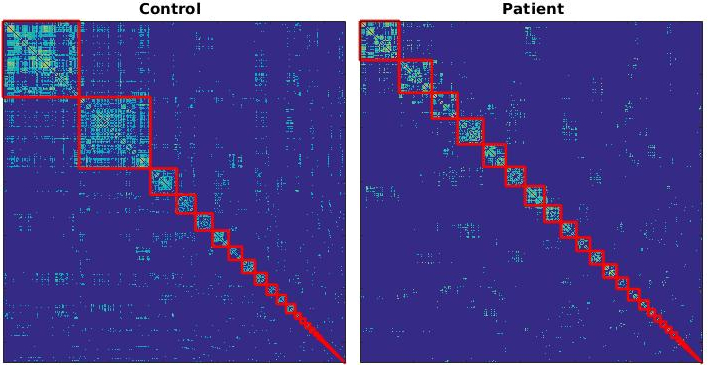
\includegraphics[width=\textwidth]{images/schizo/schizo_fig_3.jpg}
\caption{Optimal Asymptotical Surprise partitions for the two populations.}
\label{fig:schizo_control_patients}
\end{figure}

Figure~\ref{fig:schizo_figure5} shows the distribution of functional modules in the two groups overlaid on an anatomical template.
Note that the colors denoting the communities were chosen independently in the two groups to maximize contrast between adjacent modules.
Differences in the modular structures of functional connectivity in the two groups are apparent, and involve complex reorganization of nodal membership across modules.
The main differences in modular organization between the two groups involve the sensorimotor, visual and auditory cortices.
The large central module in the healthy controls' group (dark blue in Figure~\ref{fig:schizo_figure5}A) comprises somatosensory cortices and temporal auditory cortices, consistent with previous findings in healthy volunteers~\cite{javitt2015}.
In schizophrenia patients, this module breaks up into four different clusters of nodes.
Similarly, the controls' large occipital module (light brown in Figure~\ref{fig:schizo_figure5}) is split in the patients' group, with primary visual cortex standing as an independent community together with part of the inferior temporal lobe.
The more dorsal part of the occipital community includes part of the superior parietal lobule in HCs, but not in SZ patients, where the boundary of this community lies in the vicinity of the parieto-occipital fissure.

\begin{figure}
\centering
    \begin{tabular}{c}
    \textbf{\textsf{A. Controls}} \\
	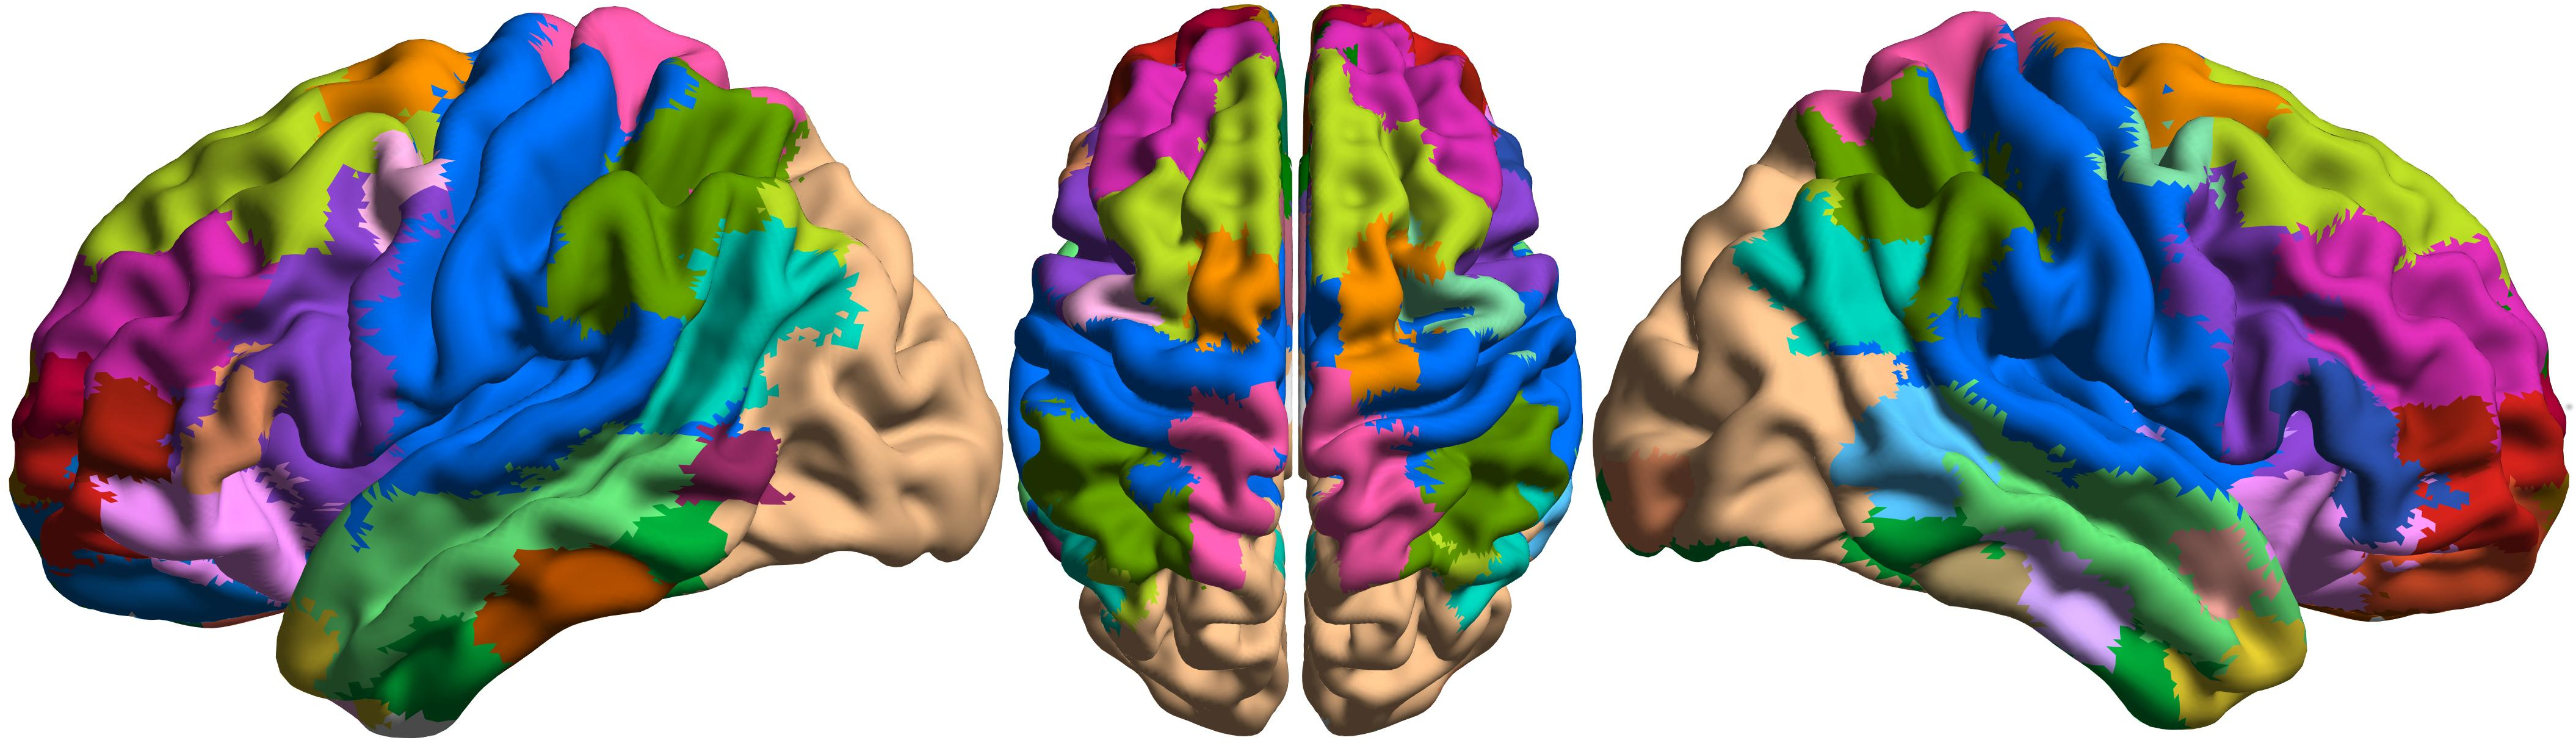
\includegraphics[width=0.75\textwidth]{images/schizo/schizo_fig_5a.jpg} \\
	\textbf{\textsf{B. Patients}} \\
	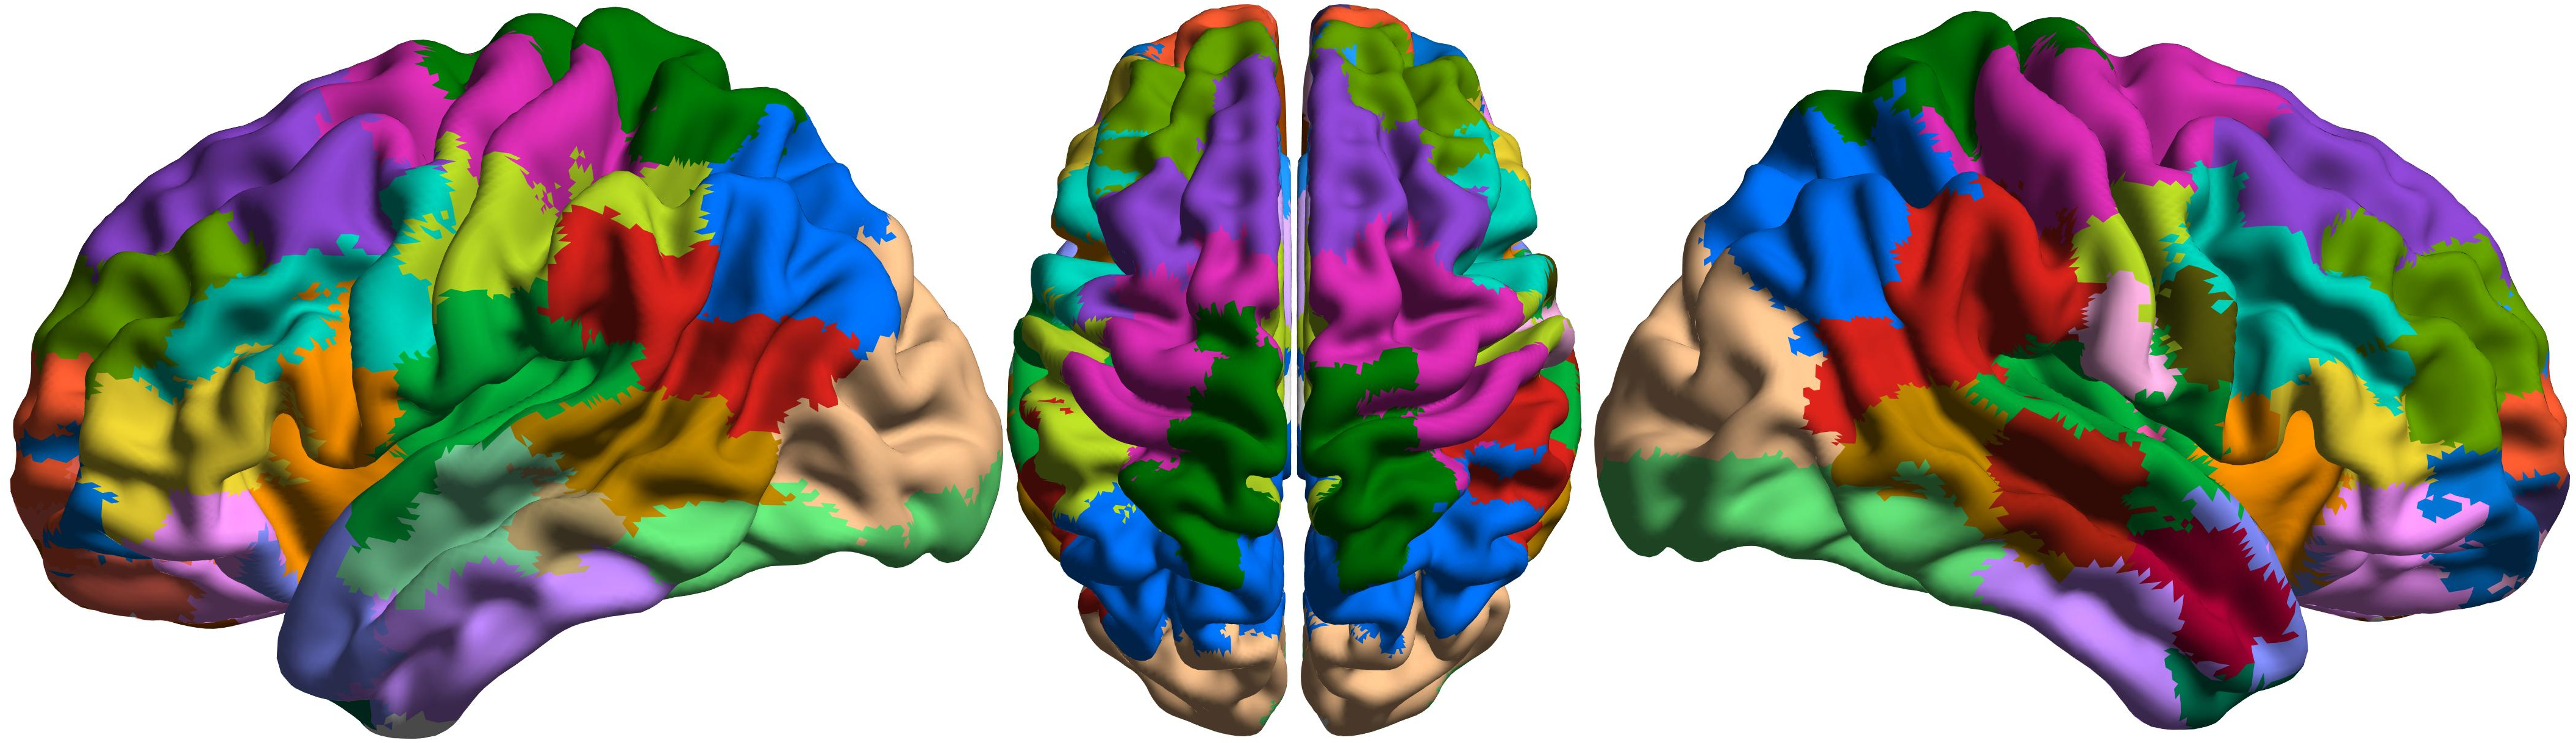
\includegraphics[width=0.75\textwidth]{images/schizo/schizo_fig_5b.jpg} \\
	\end{tabular}
\caption{Maps representation of the communities for each group: A. Healthy control, B. Schizophrenia patient. Please note that the colors of each community are random even across group.}
\label{fig:schizo_figure5}
\end{figure}

Substantial fragmentation and reorganization is also observed in the modular structure of the temporal cortex.
In controls, we find well-delineated modules comprising the middle temporal gyrus and the inferior temporal gyrus, while the superior temporal gyrus is part of larger community that includes somatosensory cortices.
In patients, the superior temporal gyrus is separated from the larger somatosensory community, and is split into two modules, anterior and posterior, respectively, that comprise also part of the supramarginal cortex.
The middle temporal gyrus is split rostrocaudally into 4 different communities that include parts of the superior and inferior gyri.
The inferior gyrus is split in ttwo modules, anterior and posterior, respectively.
The anterior module includes part of the middle temporal gyrus, while the posterior one extends to visual cortices. 

Interestingly, the angular gyrus and the supramarginal gyrus appear as separate modules in healthy controls, but in patients these areas are merged into a single community including the temporoparietal junction. 
Finally, between-group differences in frontal lobe organization pertain particularly the language regions, with the Broca area forming an independent community in patients.
The modular structure of other frontal and prefrontal areas is consistent in the two groups.

Figure~\ref{fig:schizo_figure6} shows statistically significant voxelwise differences in participation coefficient, a measure of diversity in intermodular connections of individual nodes.
Nodes characterized by high participation coefficients have many links pointing to different modules, and are thought to play an integrative role. 
Conversely, nodes with most links pointing to other nodes within the same community are dubbed provincial hubs, and contribute to defining functional segregation of their communities.
Significantly larger participation coefficients are observed observed in sensorimotor, visual and auditory areas of SZ patients.
Conversely, lower participation coefficients in patients are observed in frontal and parietal regions, with the most prominent decrease in the temporal primary auditory cortex in the vicinity of the Heschl gyrus.
Substantial differences are also observed in functional connectivity of areas related with language generation and processing.

The anterior part of the Broca area (Brodmann area 45), which receives afferent projections from the PFC, shows a decrease in participation coefficient, while the posterior part (Brodmann area 44), which has more structural connections with sensory cortices and inferior parietal cortices, shows an increase in PC. 

\begin{figure}[t!]
\centering
    \begin{tabular}{c}
    \textbf{\textsf{A. SCZ > CON}} \\
    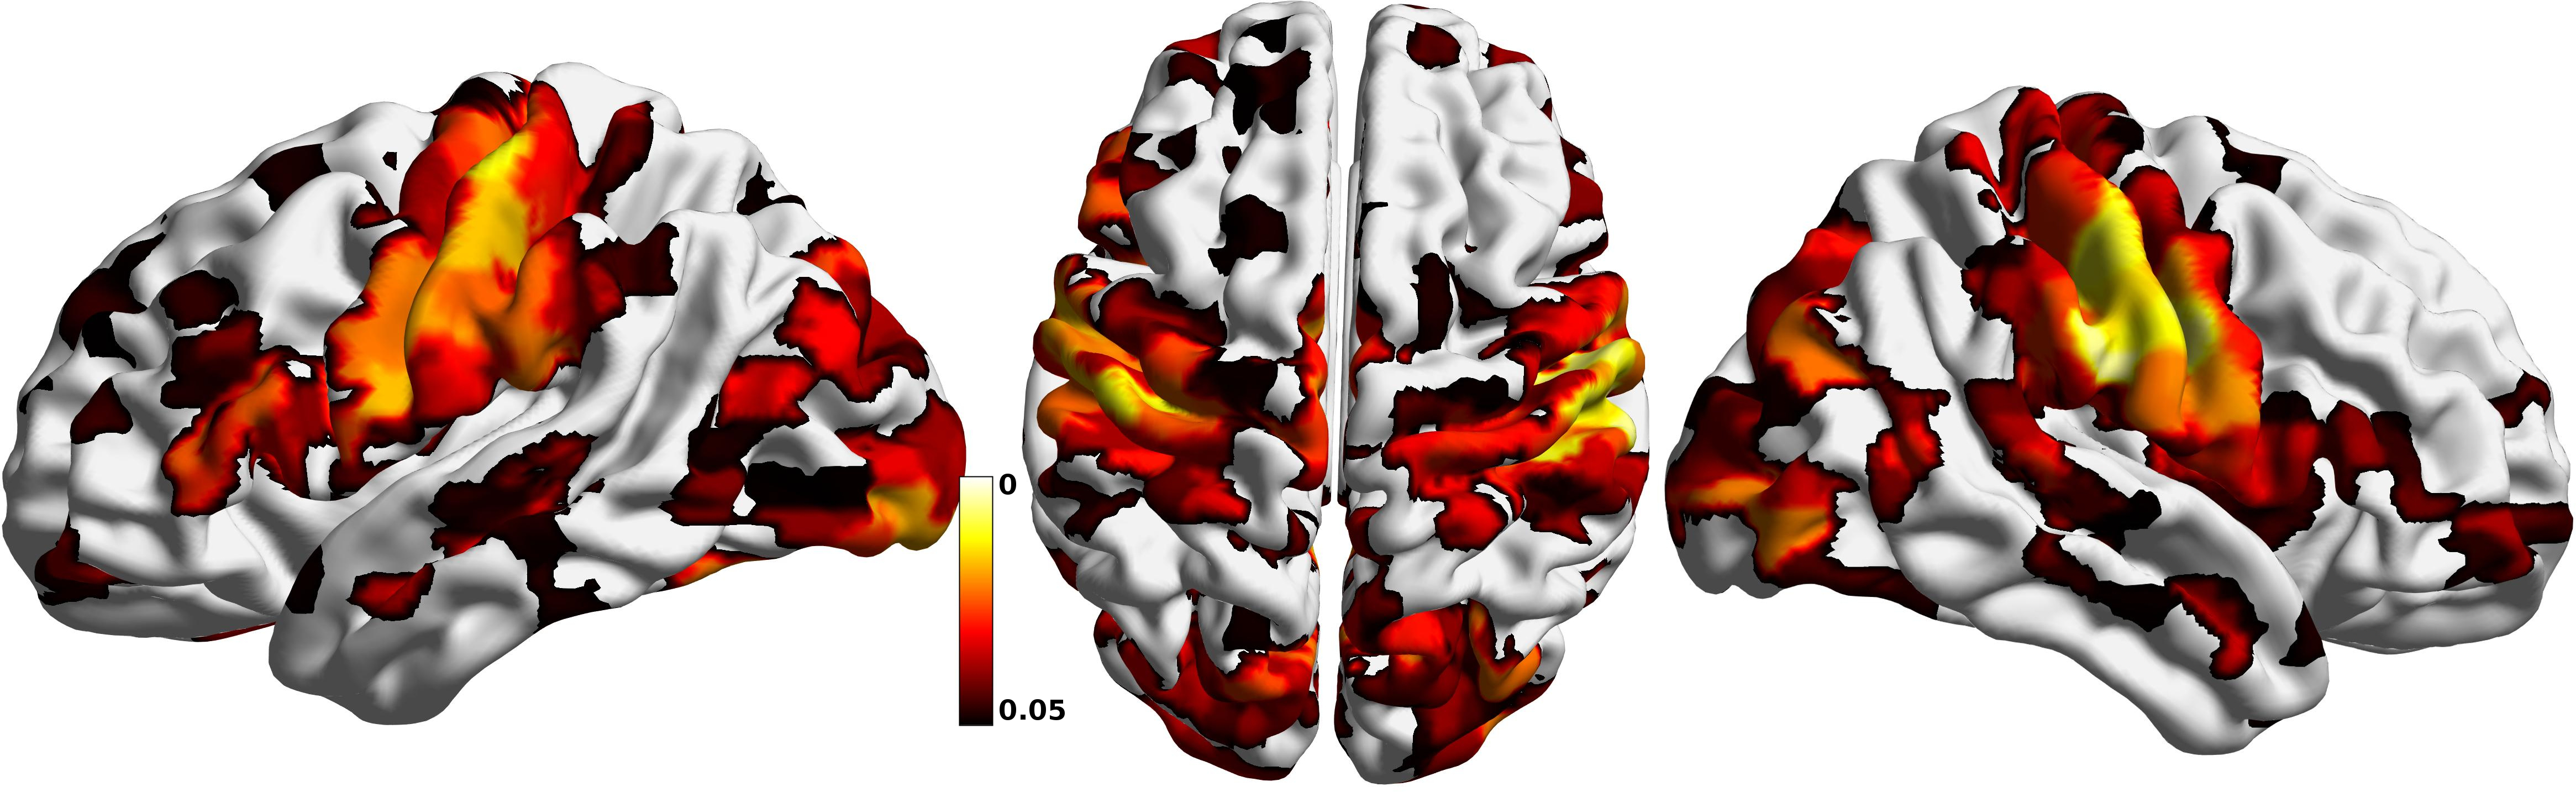
\includegraphics[width=0.75\textwidth]{images/schizo/Schizo_PatientGreaterParticipation_3views.jpg} \\
    \textbf{\textsf{B. CON > SCZ}} \\
    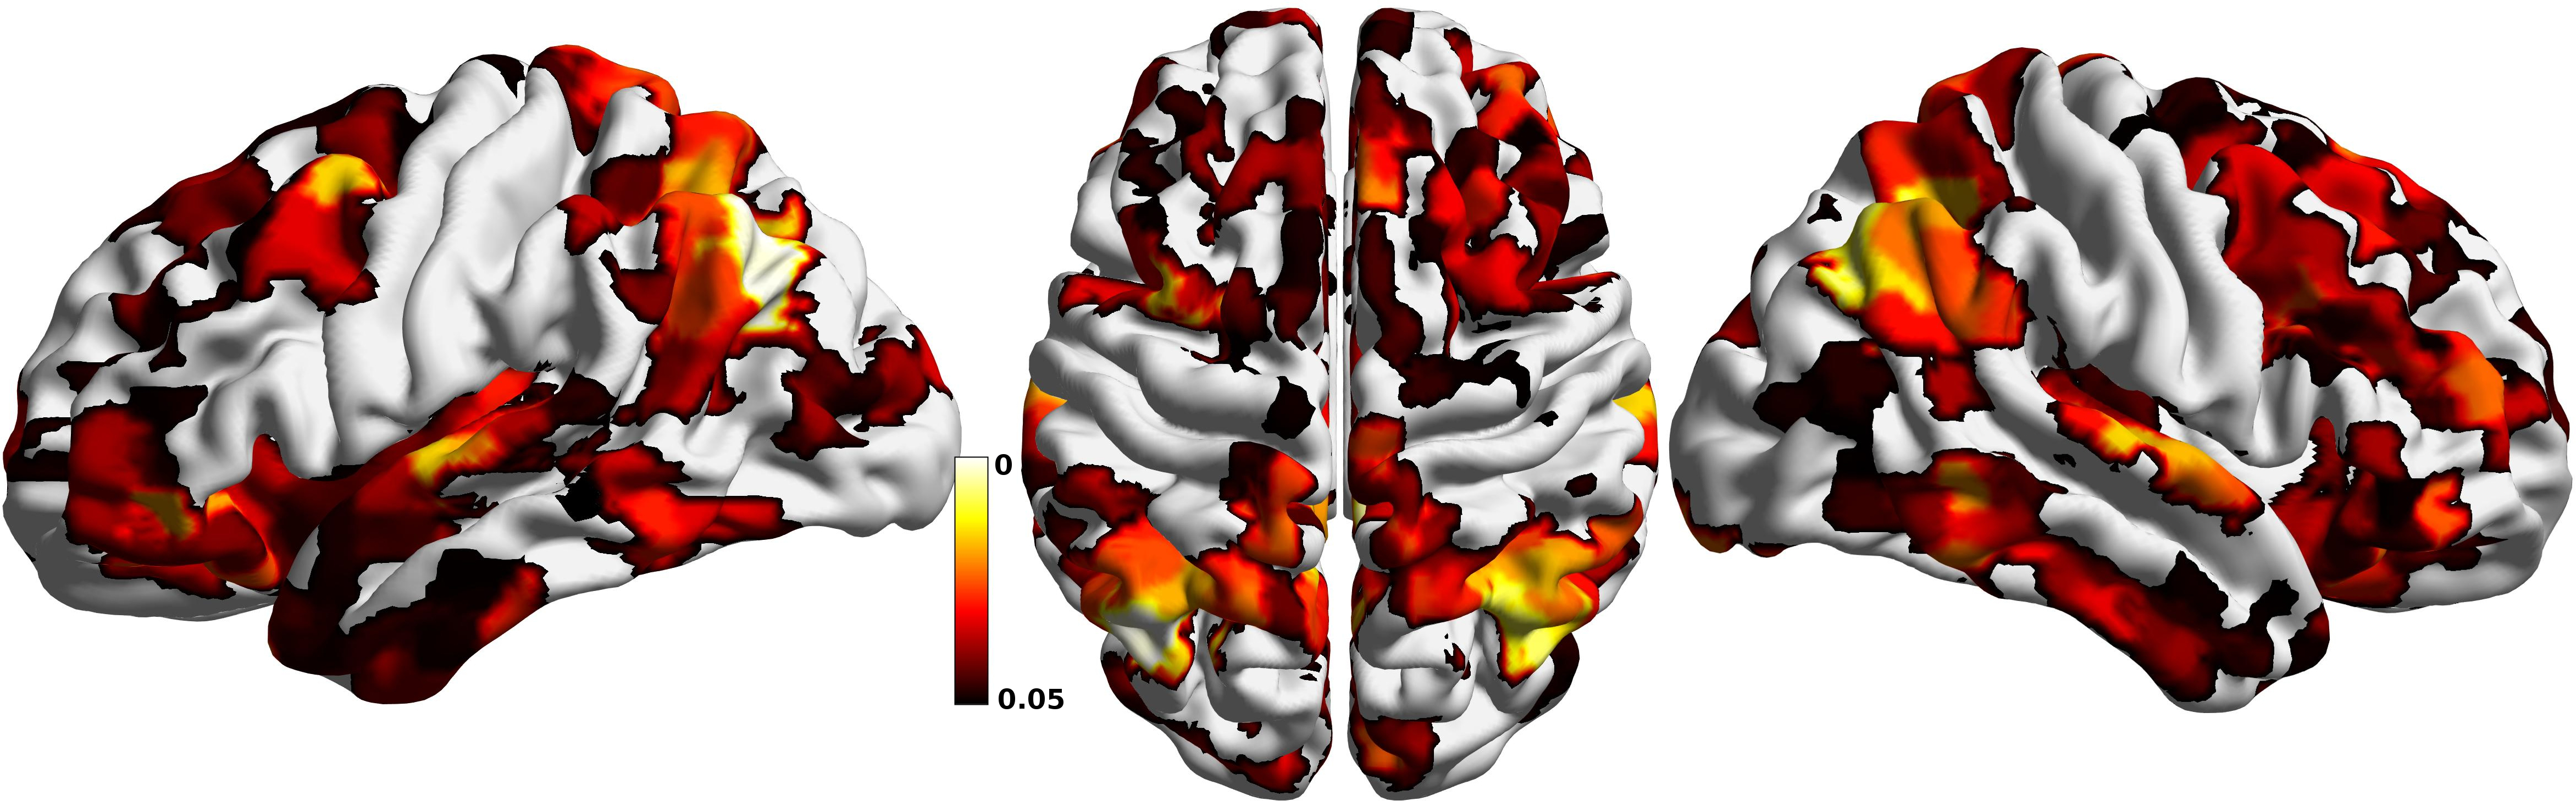
\includegraphics[width=0.75\textwidth]{images/schizo/Schizo_PatientLessParticipation_3views.jpg}
    \end{tabular}
\caption{Participation coefficient map of the difference between the two populations. a. Nodes with higher participation coefficient in SCZ than for CON; b. Nodes with lower participation coefficient in SCZ than for CON.}
\label{fig:schizo_figure6}
\end{figure}

Network nodes characterized by high degree and high participation coefficient represent the integrative hubs of connectivity networks, and are dubbed ``connector hubs''.
Differences in centrality and connectivity structure between the two populations may result in a different distribution of connector hubs in the brain.
Figure~\ref{fig:schizo_figure7} shows the regions with simultaneously high values of degree and participation coefficient in the SZ and healthy control groups.
Notable differences are observed in the parietal regions, where the superior parietal lobule represents a connector hub in control subjects, but not in patients. Importantly, the Broca area appears as prominent connector hub only in the SZ subjects.

\begin{figure}[t!]
\centering
    \begin{tabular}{c}
    \textbf{\textsf{A. Controls}} \\
    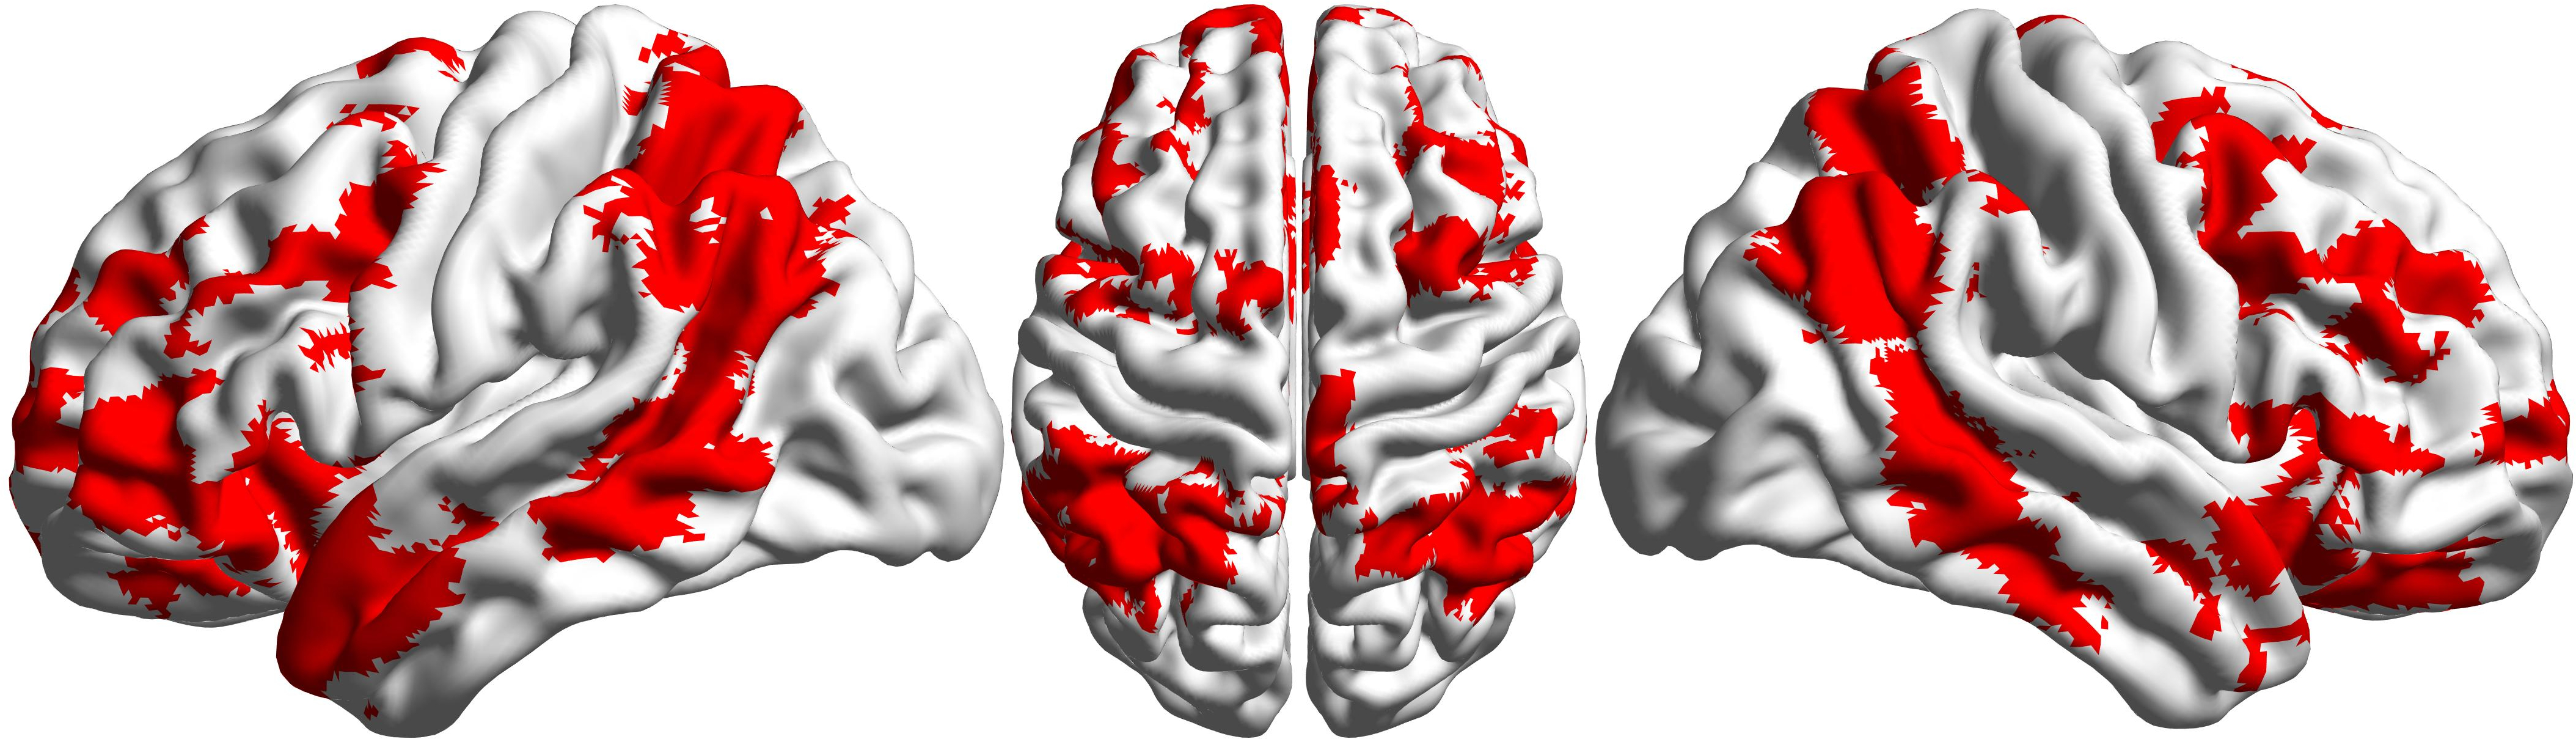
\includegraphics[width=0.75\textwidth]{images/schizo/SchizoControl_Surprise_MaskPat_0-6_Deg_1.jpg} \\
    \textbf{\textsf{B. Patients}} \\
    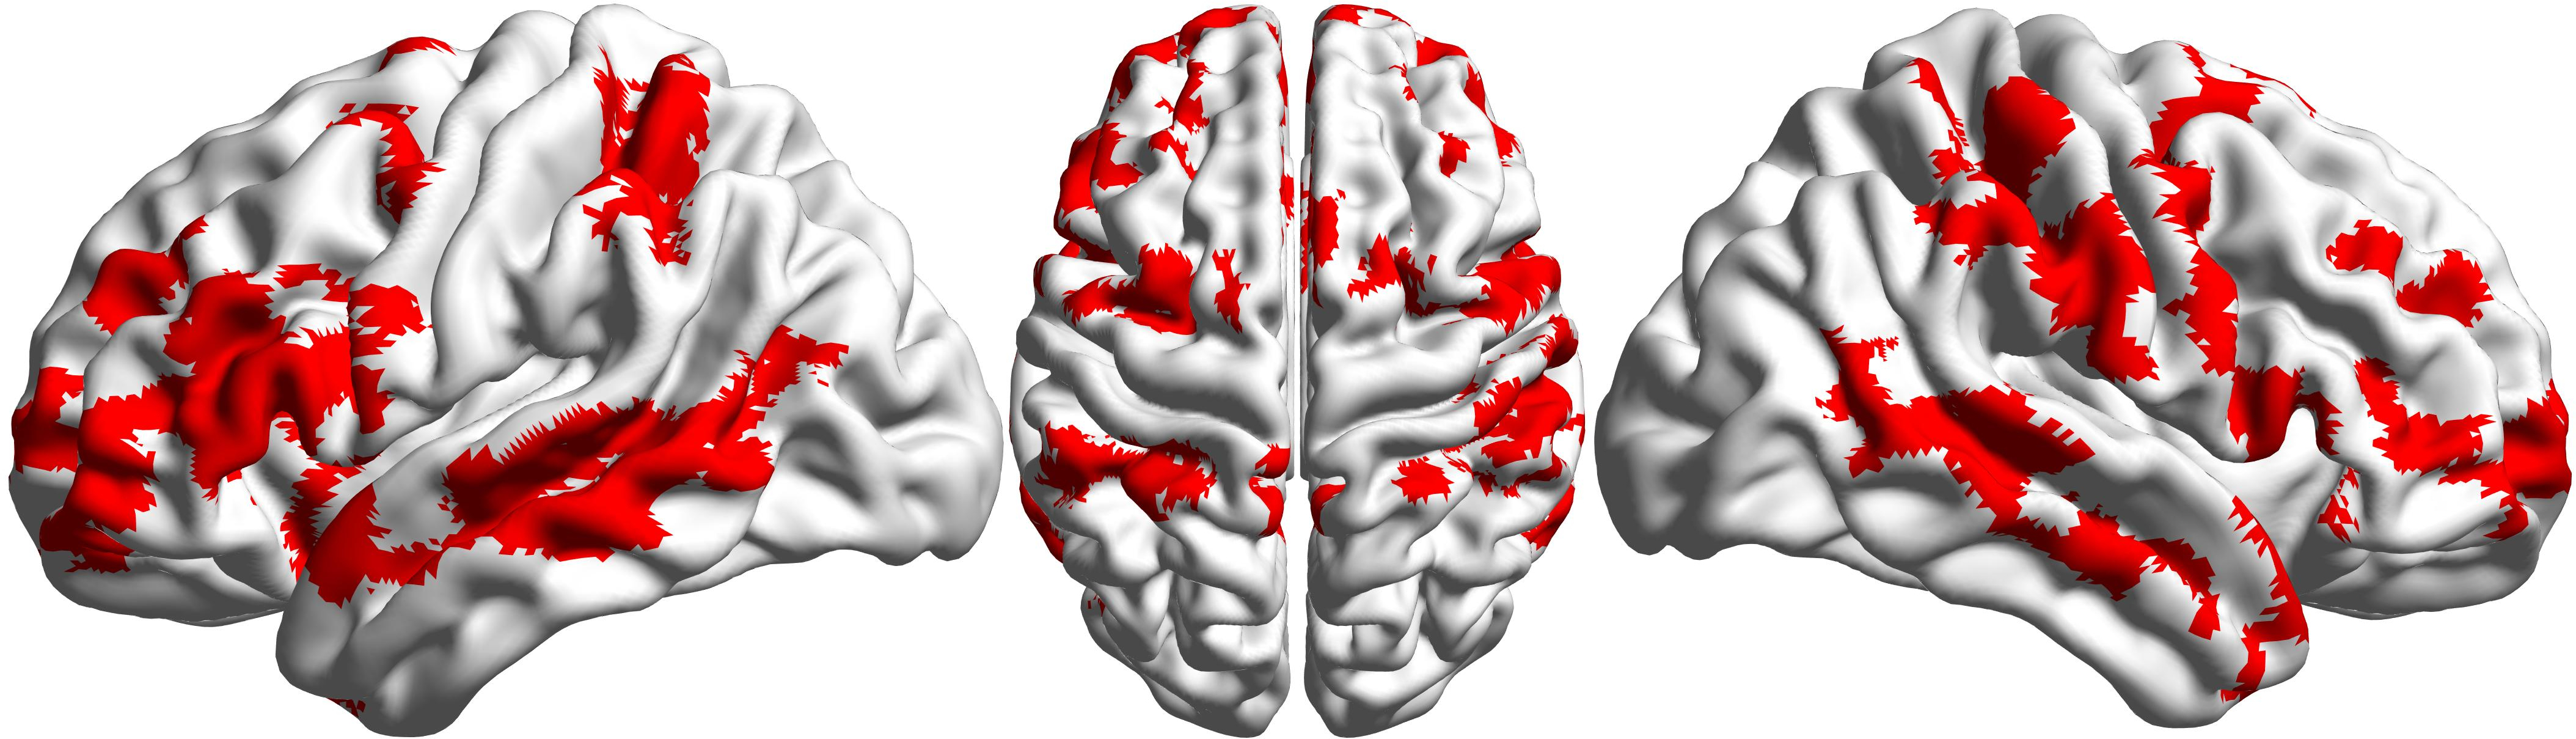
\includegraphics[width=0.75\textwidth]{images/schizo/SchizoPatient_Surprise_MaskPat_0-6_Deg_1.jpg}
    \end{tabular}
\caption{Maps of connector hubs with a participation coefficient higher than 0.6 and a degree higher than 1 for both populations.}
\label{fig:schizo_figure7}
\end{figure}

To get an idea of the main changes due to the difference of network, we looked at the participation coefficient of the nodes.
This information points out the changes of node role in the different population, i.e. when nodes get important because of its links towards the other communities.
As shown on Figure~\ref{fig:schizo_figure7}, the nodes of the motor cortex of the patient group increase their participation coefficient in the inter-community connection when conversely, the parietal as well as some frontal and temporal nodes reduce the importance of their external links compared to the second groups.

In summary, the modular structure of functional connectivity is substantially reorganized in SZ patients, with prominent differences involving primary sensory and sensorimotor areas, and language related areas. 

% \section{Discussion}
% Alterations in sensory experience and processing have been documented for a long time~\cite{bleuler1911,mcghie1961}, but studies in schizophrenia have traditionally focused on deficits in higher-order processes such as working memory and executive function.
% It has been suggested that bottom-up deficits in cognitive processing may be driven by impairments in basic perceptual processes that localize to primary sensory brain regions~\cite{javitt2009,javitt2009a}.
% The major reorganization of functional connectivity in sensory areas hereby reported is in keeping with the idea that disorders in schizophrenia may occur already at the level of early sensory processing.
% By way of example, dysfunction in auditory sensory processing has been consistently observed in schizophrenia with the auditory mismatch negativity (MMN) test~\cite{javitt2015}, and have been related with altered intrinsic and extrinsic connectivity in the Superior Temporal Gyrus~\cite{garrido2008}, consistent with our observations.
% Moreover, fragmentation of connectivity within the sensorimotor and auditory cortex module is consistent with deficits in sensorimotor gating such as those observed in SZ patients by Pre Pulse Inhibition tests~\cite{braff1990}.

% One hypothesis for this particularity might be proposed observing the node betweenness centrality of the network.
% Indeed, this index represents the fraction of all shortest paths in the network that contain a given node.
% In our case, the Schizophrenia group exhibits an average betweenness centrality of $1787\pm 2636$ when the healthy group is at $1104 \pm 1673$.
% By definition, nodes with high values of betweenness centrality participate in a large number of shortest paths.
% This suggests that the patients are balancing their weaker long distance connectivity by increasing their number of shorter paths.

% At a more fundamental level, a problem exists with the comparison of connectivity networks from different groups of subjects characterized by different connectivity strengths.
% Typically, functional connectivity networks are constructed on the basis of interregional correlations in the BOLD signal for the definition of the graph edges.
% Sparsification procedures are applied to remove the weaker edges, thus reducing the effects of noise and improving detection of the modular structure of connectivity graphs.

% A critical issue is hence the determination of the optimal threshold to cut off (reduce) weaker edges, while maintaining the essential features of the network's structure~\cite{alexander-bloch2010}.
% In most cases, including previous studies in Schizophrenia subjects, thresholds were adjusted to ensure the same density of edges for the group level networks representing patients and controls.
% However, as pointed out by van den Heuvel and Fornito~\cite{vandenheuvel2014}, this approach may be inappropriate when comparing groups with different connectivity strength.
% Indeed, if patients show inherent reduction in connectivity, equalizing the edge density to that of the control group will introduce a higher proportion of spurious correlations, thus resulting in a network with a more random topology~\cite{fornito2012}. To what extent this bias has affected recent cross-sectional studies in schizophrenia remains to be elucidated.

% Moreover, we demonstrate that percolation analysis~\cite{stauffer1994,gallos2012}, a method used in statistical physics to assess the robustness of network structure, provides a means to calculate the optimal threshold that maximizes the information retrieved by Surprise.
% This procedure overcomes the pitfall of imposing constant edge density to networks with different connectivity strengths, and enables rigorous between-group comparisons.

%%%%%%%%%%%%%%%%%%%%%%%%%%%%%%%%%%%%%%%%%%%%%%%%%%%%%%%%%%%%%%%%%%%%%%
%%%%%%%%%%%%%%%%%%%%%%%% PERCOLATION ANALYSIS %%%%%%%%%%%%%%%%%%%%%%%%
%%%%%%%%%%%%%%%%%%%%%%%%%%%%%%%%%%%%%%%%%%%%%%%%%%%%%%%%%%%%%%%%%%%%%%
\section{Conclusions}
In conclusion, we have applied a novel graph theoretical approach, dubbed Asymptotical Surprise, to study the structure of brain functional connectivity networks in a large cohort of Schizophrenia patients.
Global and node-wise connectivity parameters show an overall reduction in connectivity in patients compared to healthy controls, in line with previous studies.
The improved resolution afforded by our method reveals substantial reorganization of the modular structure of functional connectivity in patients, with a fragmentation of visual, auditory and sensorimotor cortices.
This evidence is in keeping with bottom-up theories that posit that cognitive dysfunction and conscious disintegration observed in SZ may arise from deficits occurring already at early stages of sensory processing.
The reorganization of auditory and language modules, and the merging with multimodal association cortices is interesting in the light of the auditory hallucinations often experienced by SZ patients.
Significant changes were observed in the participation coefficient of sensory, visual, and in primary auditory cortices, including the Heschl gyrus, a region critically implicated in auditory hallucinations.
This evidence indicates that these regions play a different role in the integration of the network of functional connectivity in the patient's brain.
Previous studies using similar, but resolution-limited methods, may have failed to detect the abnormal organization of functional connectivity at the scale reported here due to intrinsic methodological limitations.
The present approach may provide a novel and powerful tool to study alterations in the brain functional organization in other neuropsychiatric conditions that are thought to be associated with aberrant connectivity.

%%%%%%%%%%%%%%%%%%%%%%%%%%%%%%%%%%%%%%%%%%%%%%%%%%%%%%%%%%%%%%%%%%%%%%
%%%%%%%%%%%%%%%%%%%%%%%% PERCOLATION ANALYSIS %%%%%%%%%%%%%%%%%%%%%%%%
%%%%%%%%%%%%%%%%%%%%%%%%%%%%%%%%%%%%%%%%%%%%%%%%%%%%%%%%%%%%%%%%%%%%%%
% \subsection{Percolation Analysis}
% For community detection, procedures are often applied to remove the weaker edges in the network, thus sparsifying the network and reducing the effects of noise. Here, we have used percolation analysis derived from statistical physics \todo{(18, 38, 39)} to identify the optimal cut-off.
% This approach measures the size of the largest connected component of the network upon iterative removal of the weakest edges and enables data-driven determination of the optimal threshold that preserves network structure and connectedness while removing potentially spurious correlations.

% To validate the use of percolation analysis to define the optimal sparsification threshold, we generated synthetic networks based on the Lancichinetti-Fortunato-Radicchi (LFR) algorithm~\cite{lancichinetti2008}.
% LFR networks provide model graphs that replicate the distribution of nodal degree observed in brain functional connectivity networks, and are endowed with a ground-truth modular structure against which the results of community detection algorithms can be assessed.

% The planted modules had sizes sampled from a power-law distribution to mimic the heterogeneous distribution of modules that is observed in functional connectivity networks~\cite{power2011,meunier2010}.
% Optimization of Asymptotical Surprise was applied to detect the community structure of the LFR networks after application of different thresholds.

% The correspondence between the partition detected by Asymptotical Surprise and the ground-truth structure was assessed by calculating the Normalized Mutual Information (NMI), an information-theoretic measure of similarity.
% Moreover, we assessed Sensitivity and Specificity, defined on the basis of true and false positives or negatives in the assignment of node membership.

% The results of this analysis for 5 instances are shown in Figure~\ref{fig:schizo_percolation}.

% The shaded zone represents the average value of the optimal threshold determined by percolation analysis for representative LFR networks with a topological mixing coefficient $\mu_t=0.4$.
% A range of different values of µt was explored, and the results are reported in the Supplementary Information section\todo{SI?}.
% The graphs reveal that the threshold obtained by percolation analysis corresponds to the maximum value of NMI, thus maximizing the correspondence between the retrieved and ground-truth modular structure.
% Moreover, the percolation threshold falls in a range where both Specificity and Sensitivity are at their highest~\cite{zahoranszky-kohalmi2016a}, thus providing the best quality partition.
% Additionally, we have injected different levels of noise in the correlation structure of the LFR matrix to simulate the effects of data variability\todo{SI?}.
% Consistently with the idea that weaker edges are more vulnerable to the effects of data variability, and reduce the ability to recover the planted structure, we found that Asymptotical Surprise performed best with networks sparsified using percolation analysis.

% Alterations of the modular organization of functional connectivity should not be interpreted as a redefinition and remapping of functionally specialized areas, as identified in task-related functional MRI studies.
% Indeed, community detection in resting state functional connectivity networks assesses topology and strength of the interactions between functionally segregated regions.

% \paragraph{Asymptotical Surprise}
% The algorithm that we chose, to determine community structure in our two groups, is named Asymptotical Surprise, a conceptually different fitness function grounded in probability theory. It was maximized with PACO (Partitioning Cost Optimization) algorithm~\cite{nicolini2016,nicolini2017}.

% Our decision was based on the ability of this method, considered as resolution limit free, to reveal complex modular structure of resting state connectivity, with communities of widely different sizes reflecting distributed functional networks alongside with small, functional defined modules. In resume it allows us a more fine and detailed representation of the modular structure of our population.
% The Matlab toolbox to obtain the community structure with Surprise is available at \url{http://forms.iit.it/view.php?id=68447}.

% \paragraph{Percolation analysis}

% Prior to analyzing the network with Asymptotical Surprise, it is common procedure to apply a threshold on the adjacency matrix. 
% The idea is to discard edges with low weight, in order to reduce the effect of noise by sparsifying the matrix. 
% We decide to use a percolation analysis approach. 
% By definition, derived from statistical physics~\cite{stauffer1994,alexander-bloch2010,gallos2012,fornito2016}, the percolation analysis identifies the number of edges that have to be removed before the giant component disappears, i.e. the network break down and co1llapse.

% In order to test this method on graph similar to the brain, we generated connectivity matrix and their ground-truth modular structures based on the idea that brain networks display modules with a heterogeneous size distribution.


% \subsection{Participation coefficient}
% To complete the investigation at the node level, we choose to consider the alteration in the nodes role between the two populations.
% The participation coefficient~\cite{guimera2005} reflects the importance of nodes regarding its inter-modular connections.
% We estimated the index of each node for each subjects.
% Finally, we ran a t-test for each node across group before to correct the obtained p-value by the number of nodes.
